\chapter{Revisão da Literatura}
\section{Algoritmos de Regressão}

Regressão é o processo de descobrir relações entre variáveis de entrada e de saída a partir de um conjunto de dados~\cite{STULP201560}. As técnicas de regressão podem ser divididas em duas categorias principais: regressão paramétrica e não paramétrica.

A regressão paramétrica fixa uma relação funcional entre as variáveis e seu objetivo é estimar os parâmetros dessa relação. Por outro lado, a regressão não paramétrica não assume uma forma funcional específica, permitindo maior flexibilidade na modelagem de dados complexos~\cite{Angelis2023}.

Algoritmos de regressão são comumente utilizados para interpolação e extrapolação de dados. Interpolação é o processo de estimar valores dentro do espaço de dados utilizados para o treinamento do modelo de regressão, enquanto extrapolação é o processo de estimar valores fora desse espaço. Diferentes algoritmos possuem propriedades diferentes em relação a suas capacidades de interpolação e extrapolação~\cite{Angelis2023}.

Existem diversas formas de implementar algoritmos de regressão, a depender do tipo de regressão desejado para o modelo. Este capítulo focará em algoritmos de regressão não paramétricos de ordem arbitrária, especificamente no algoritmo de Regressão Simbólica implementado via programação genética e grafos de igualdade. Além disso, serão abordadas comparações com outras técnicas de implementação de regressão simbólica.

\section{Algoritmos Genéticos}

Algoritmos genéticos (AGs) são uma classe de algoritmos inspirados na evolução natural, onde soluções são evoluídas ao longo de gerações para resolver problemas complexos. A ideia principal do algoritmo é simular o processo de seleção natural, no qual a pressão exercida pelo ambiente seleciona os melhores indivíduos de uma espécie. Esses algoritmos utilizam operações como seleção, cruzamento e mutação para explorar o espaço de soluções~\cite{Angelis2023,sr_book}. O objetivo principal é otimizar um objetivo arbitrário em relação a um conjunto de variáveis de entrada~\cite{Beyer2002}. Algoritmos genéticos são amplamente utilizados em problemas de busca, otimização, decisão e aprendizado de máquina~\cite{galr}.

O funcionamento básico do algoritmo segue os seguintes passos:
\begin{enumerate}
  \item Uma população inicial de soluções é gerada aleatoriamente;
  \item A cada iteração, os indivíduos da população são avaliados com base em uma função de aptidão, que indica o quão bem cada indivíduo resolve o problema;
  \item Os melhores indivíduos são selecionados para reprodução;
  \item Operadores de cruzamento e mutação são aplicados para gerar novos indivíduos;
  \item A nova população é formada com os indivíduos gerados;
  \item O processo é repetido até que um critério de parada seja atingido.
\end{enumerate}

Para implementação do algoritmo, é necessário definir a forma de representação dos indivíduos. Uma representação comumente utilizada é a codificação por cadeia de caracteres binária, na qual cada indivíduo é representado por uma sequência de bits, na qual cada bit representa uma propriedade do indivíduo~\cite{Katoch2021}. No algoritmo de regressão simbólica, abordado mais adiante, os indivíduos são representados por árvores de sintaxe abstrata, as quais codificam operações matemáticas.

\subsection{Operador de seleção}

Seleção é o processo de escolher quais indivíduos da população atual serão utilizados para reprodução. Diversas estratégias de seleção podem ser utilizadas, como seleção por torneio e roleta. A seleção por torneio envolve a escolha dos melhores indivíduos de um subconjunto aleatório da população baseando-se nos maiores valores da função de aptidão. A seleção por roleta envolve a escolha de indivíduos com base em uma distribuição probabilística, onde indivíduos com maior aptidão têm maior probabilidade de serem selecionados~\cite{Katoch2021}.

\subsection{Operador de crossover}

Cruzamento é o processo de combinação dos genomas de dois indivíduos para geração de novos indivíduos~\cite{galr,Katoch2021}. Normalmente, o cruzamento é realizado escolhendo-se um ponto aleatório de corte na representação genética dos indivíduos e trocando-se as partes dos genomas a partir desse ponto.

\subsection{Operador de mutação}

Mutação é o processo de alteração aleatória de um ou mais genes de um indivíduo para introduzir diversidade na população. O objetivo da mutação é evitar a convergência prematura para solução sub-ótimas~\cite{galr}. Assim como no cruzamento, a mutação depende da forma utilizada para codificação dos indivíduos. Em uma representação em que os genes são expressos por uma sequência de bits, a mutação pode ser realizada invertendo-se um ou mais bits aleatoriamente.

\section{Regressão Simbólica}

Regressão simbólica é uma técnica que busca encontrar expressões matemáticas que melhor descrevem a relação entre variáveis de entrada e saída em um conjunto de dados e pode ser categorizada como uma forma de regressão não paramétrica~\cite{eggp,rEGGression}. Algoritmos considerados \textit{State of the Art} para regressão simbólica utilizam algoritmos genéticos para evoluir expressões matemáticas que representam essas relações~\cite{Olivetti_de_Fran_a_2018,sr_book,eggp}. No entanto, a regressão simbólica também pode ser implementada usando outros métodos, como redes neurais e transformadores~\cite{Angelis2023}.

\subsection{Programação Genética para Regressão Simbólica}

A programação genética utilizada na regressão simbólica evolui expressões matemáticas representadas por árvores de sintaxe abstrata (ASTs). Cada nó da árvore representa uma operação matemática (adição, subtração, multiplicação, exponenciação, etc.) e as folhas representam variáveis de entrada ou constantes. A Figura \ref{fig:ast_example} ilustra um exemplo de árvore de sintaxe abstrata para a expressão $log(x/2) + 3x$.

\begin{figure}[ht]
  \centering
  \caption{Exemplo de uma árvore de sintaxe abstrata (AST) para a expressão $log(x/2) + 3x$.}
  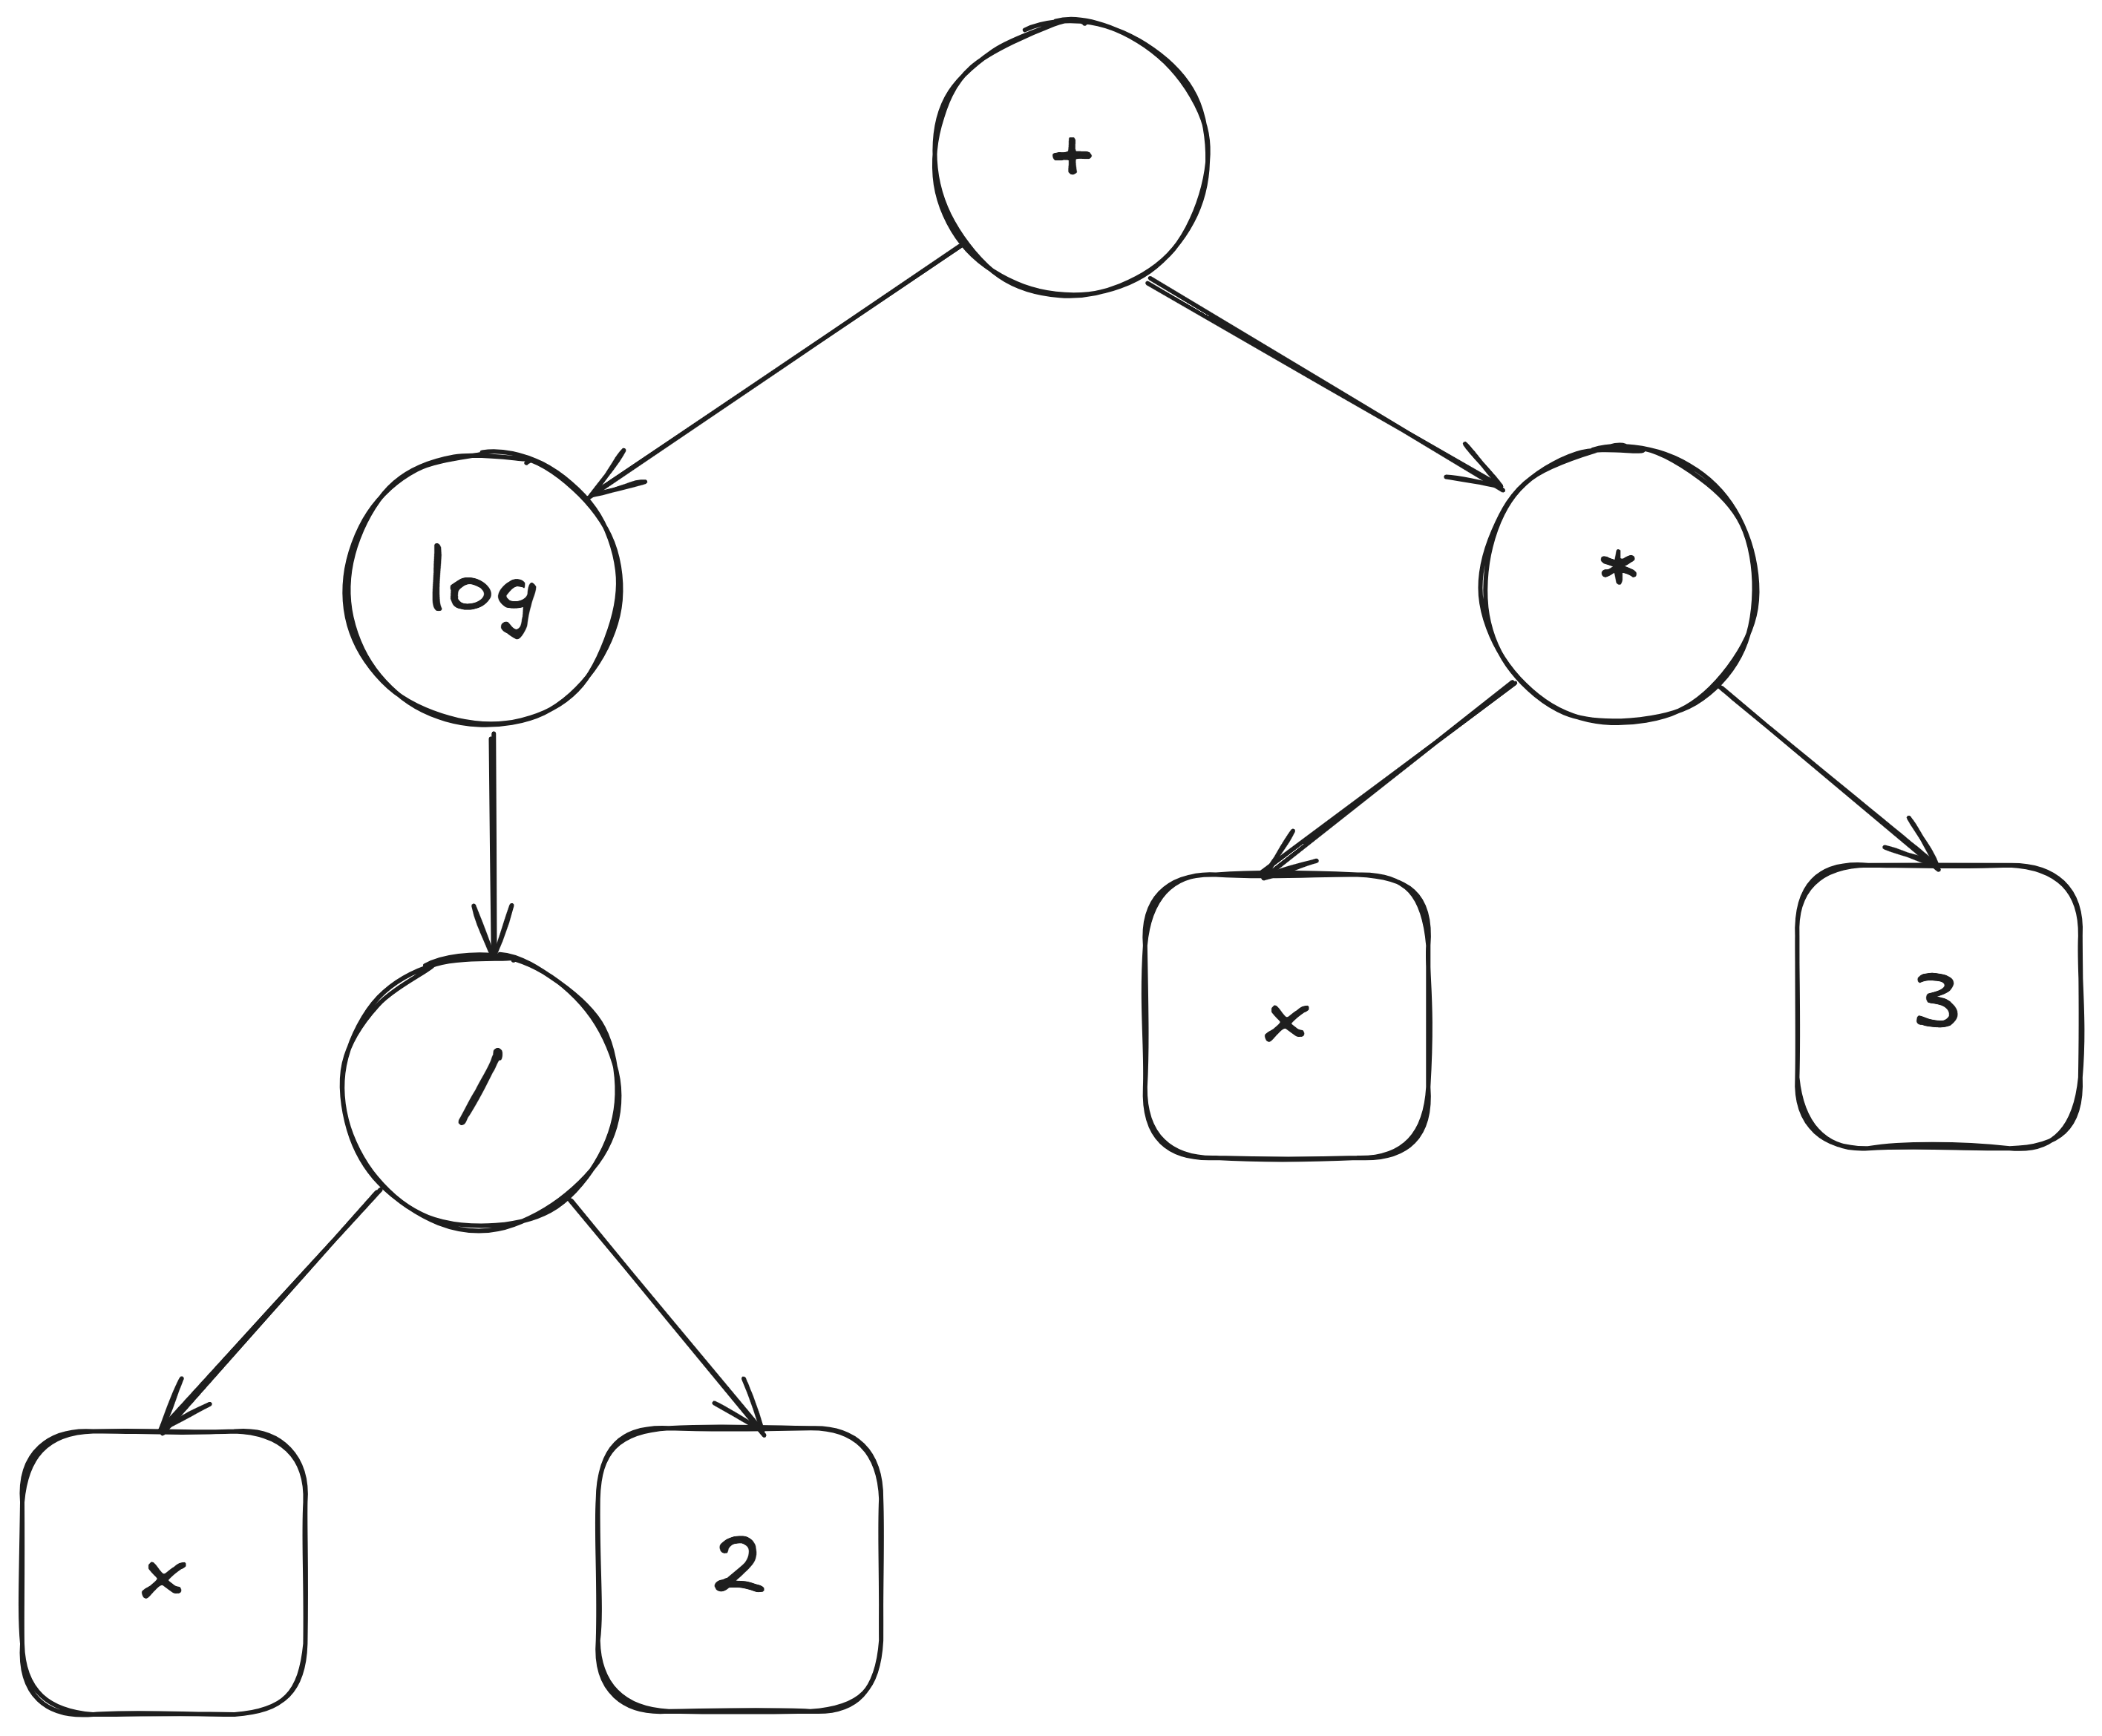
\includegraphics[width=0.5\textwidth]{images/ast_1.png}
  \label{fig:ast_example}
\end{figure}

Nós que representam operações matemáticas são representados por círculos, enquanto nós que representam variáveis de entrada ou constantes são representados por quadrados. Nós internos da árvore são chamados de não terminais, enquanto os nós folhas são chamados de terminais. O processo de busca envolve encontrar a melhor combinação de nós terminais e não terminais para minimizar a diferença entre os valores previstos pela expressão e os valores reais do conjunto de dados respeitando as restrições de complexidade e interpretabilidade da expressão~\cite{Angelis2023}.

O processo de evolução se inicia com uma população inicial de expressões aleatórias. Em cada iteração, as expressões são avaliadas com base em uma função de aptidão, que mede o quão bem cada expressão se ajusta aos dados. As melhores expressões são selecionadas para reprodução, onde passam por operações de cruzamento e mutação para gerar novas expressões que são adicionadas à nova população. Esse processo continua até que um critério de parada seja atingido. Critérios de parada comuns incluem um número máximo de gerações, obtenção da expressão ideal ou convergência da população. Comumente, uma combinação entre todos os critérios é utilizada para garantir que o processo de evolução não seja interrompido prematuramente~\cite{Angelis2023,sr_book}.

A Figura \ref{fig:ast_crossover} ilustra o processo de cruzamento entre duas expressões. Na parte superior, os indivíduos pais e, na parte inferior, os indivíduos produzidos por eles. Durante esse processo, subárvores aleatórias são selecionadas em cada expressão e trocadas entre si para criar dois novos indivíduos. Note que o cruzamento pode resultar em expressões mais complexas que os pais originais, o que pode ser controlado por meio de restrições de profundidade ou tamanho da árvore.

\begin{figure}
  \centering
  \caption{Exemplo de cruzamento entre duas expressões representadas por árvores de sintaxe abstrata (ASTs).}
  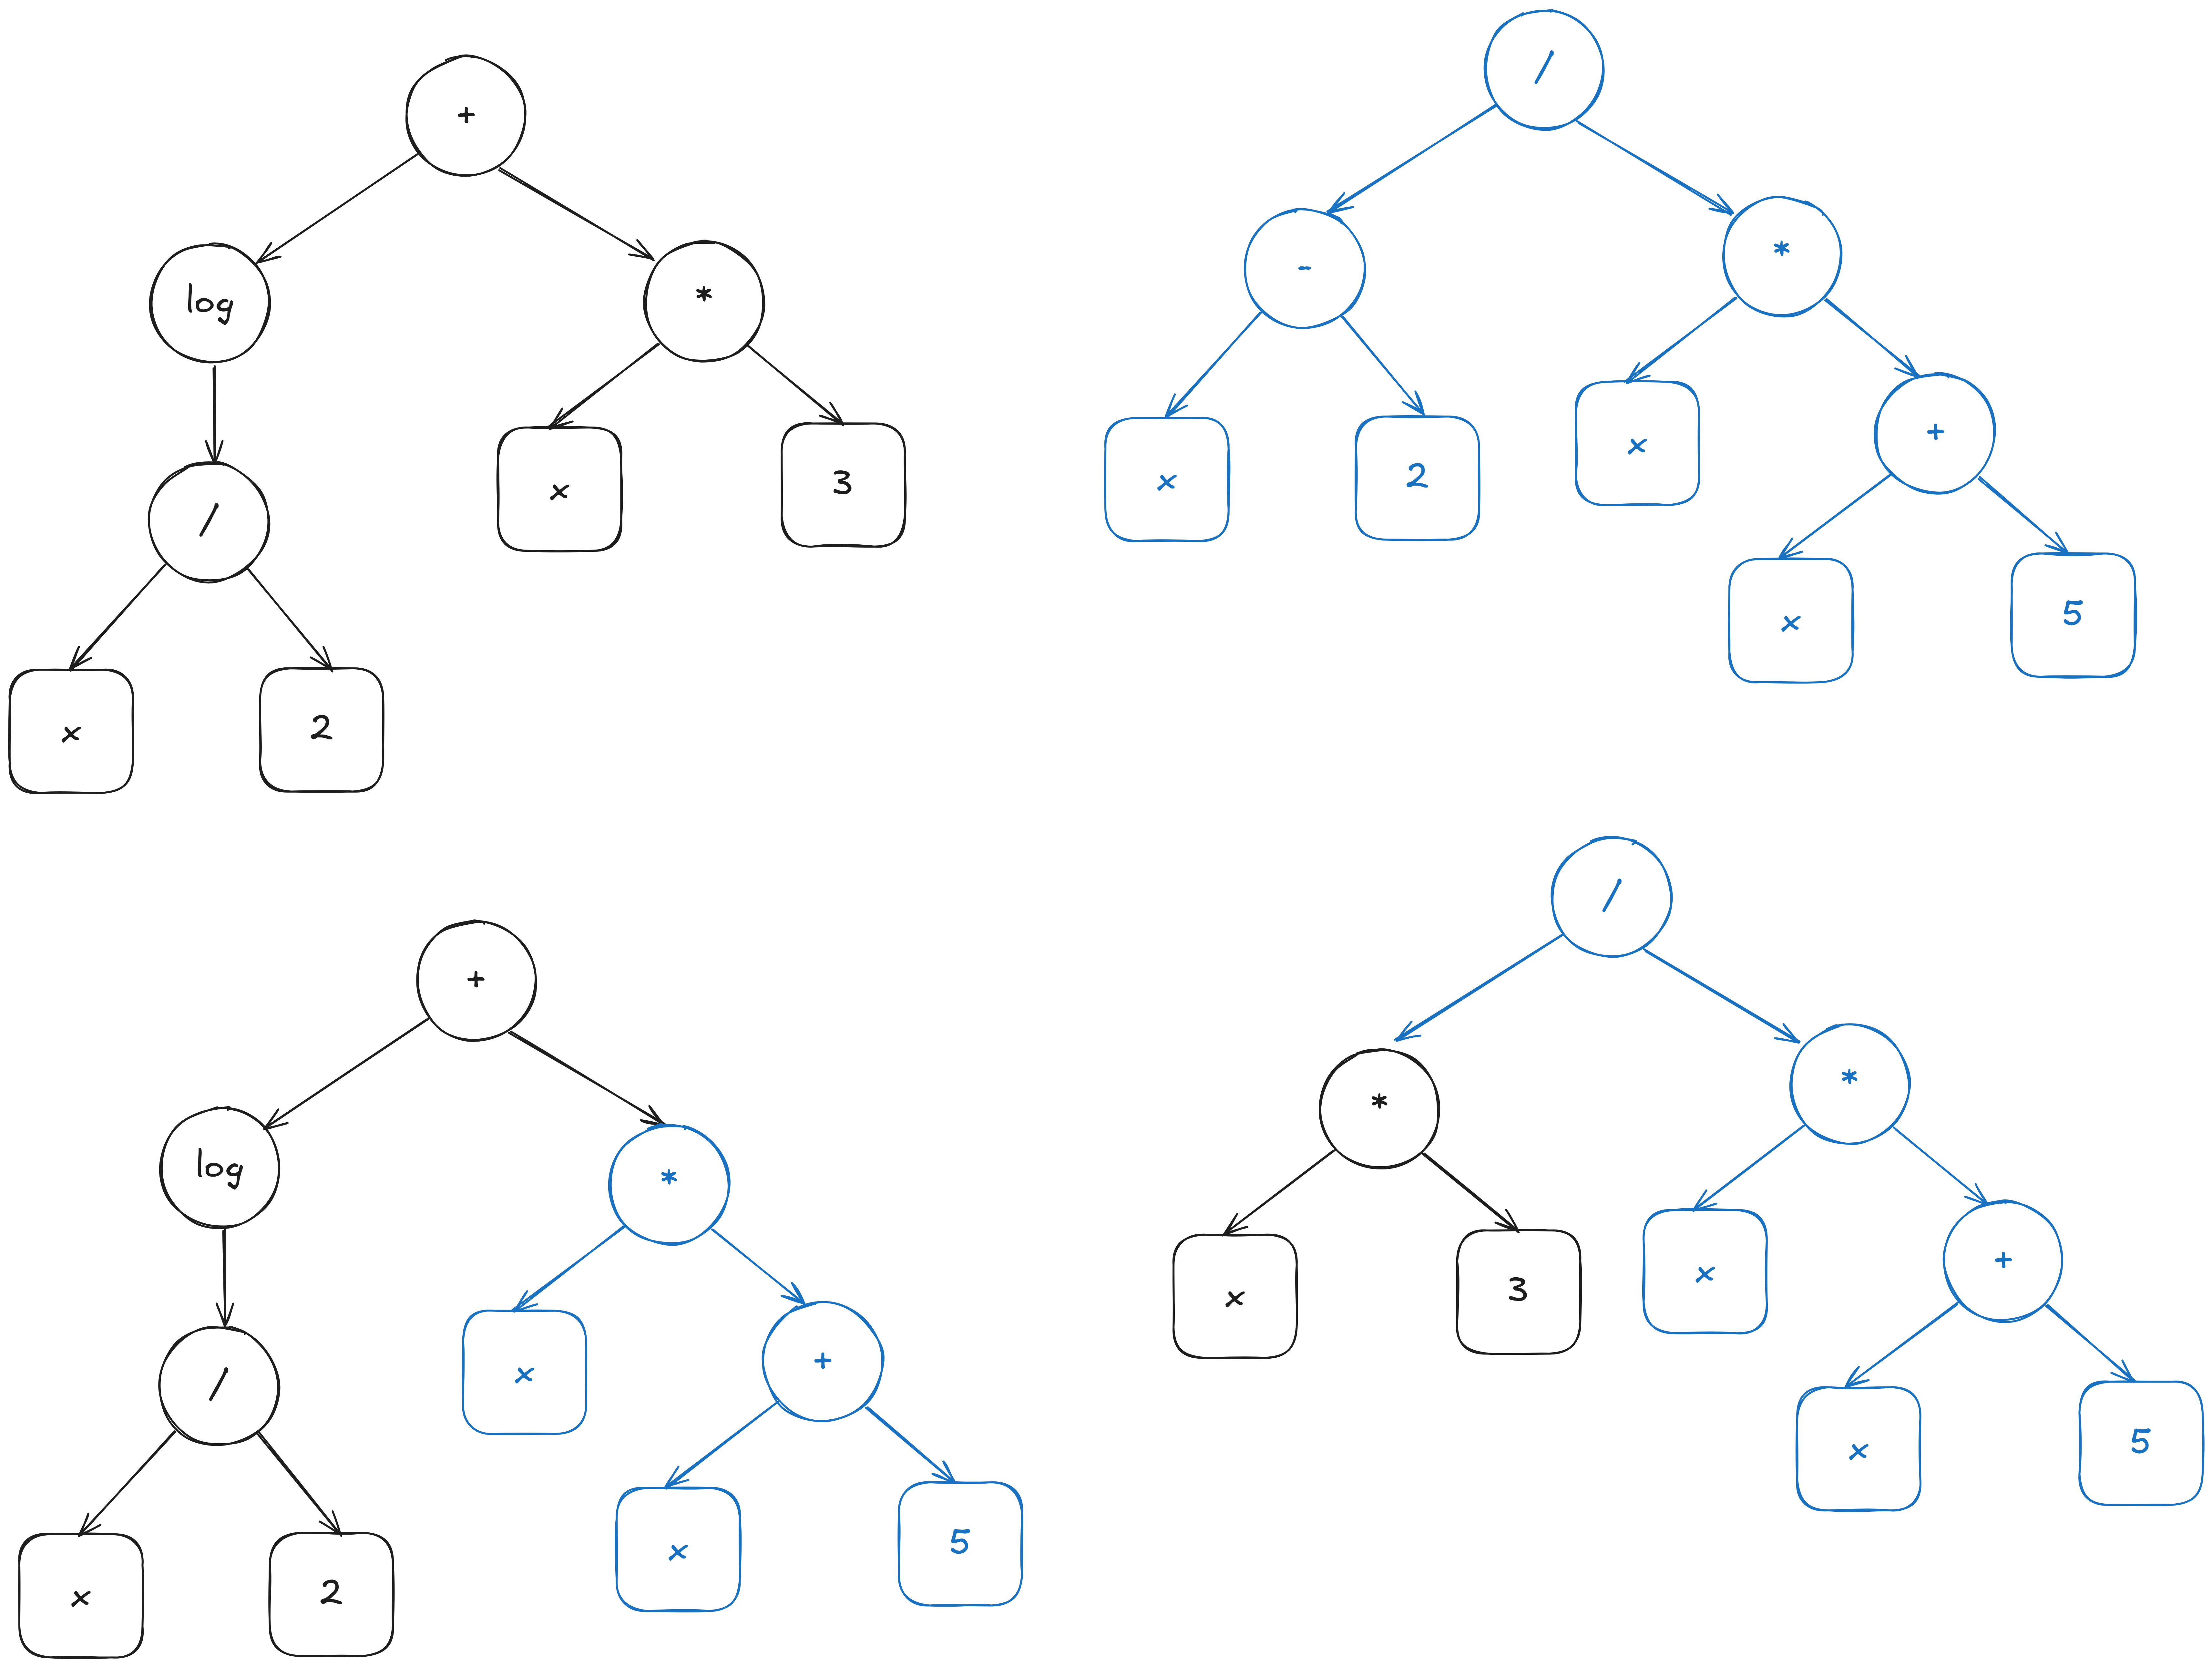
\includegraphics[width=0.8\textwidth]{images/ast_2_cross.png}
  \label{fig:ast_crossover}
\end{figure}

A Figura \ref{fig:ast_mutation} ilustra o processo de mutação, onde uma subárvore aleatória é selecionada e substituída por uma nova subárvore gerada aleatoriamente. A mutação introduz diversidade na população, ajudando a evitar a convergência prematura para soluções sub-ótimas. Na esquerda, o indivíduo original, e na direita, o indivíduo após a mutação.

\begin{figure}
  \centering
  \caption{Exemplo de mutação em uma expressão representada por uma árvore de sintaxe abstrata (AST).}
  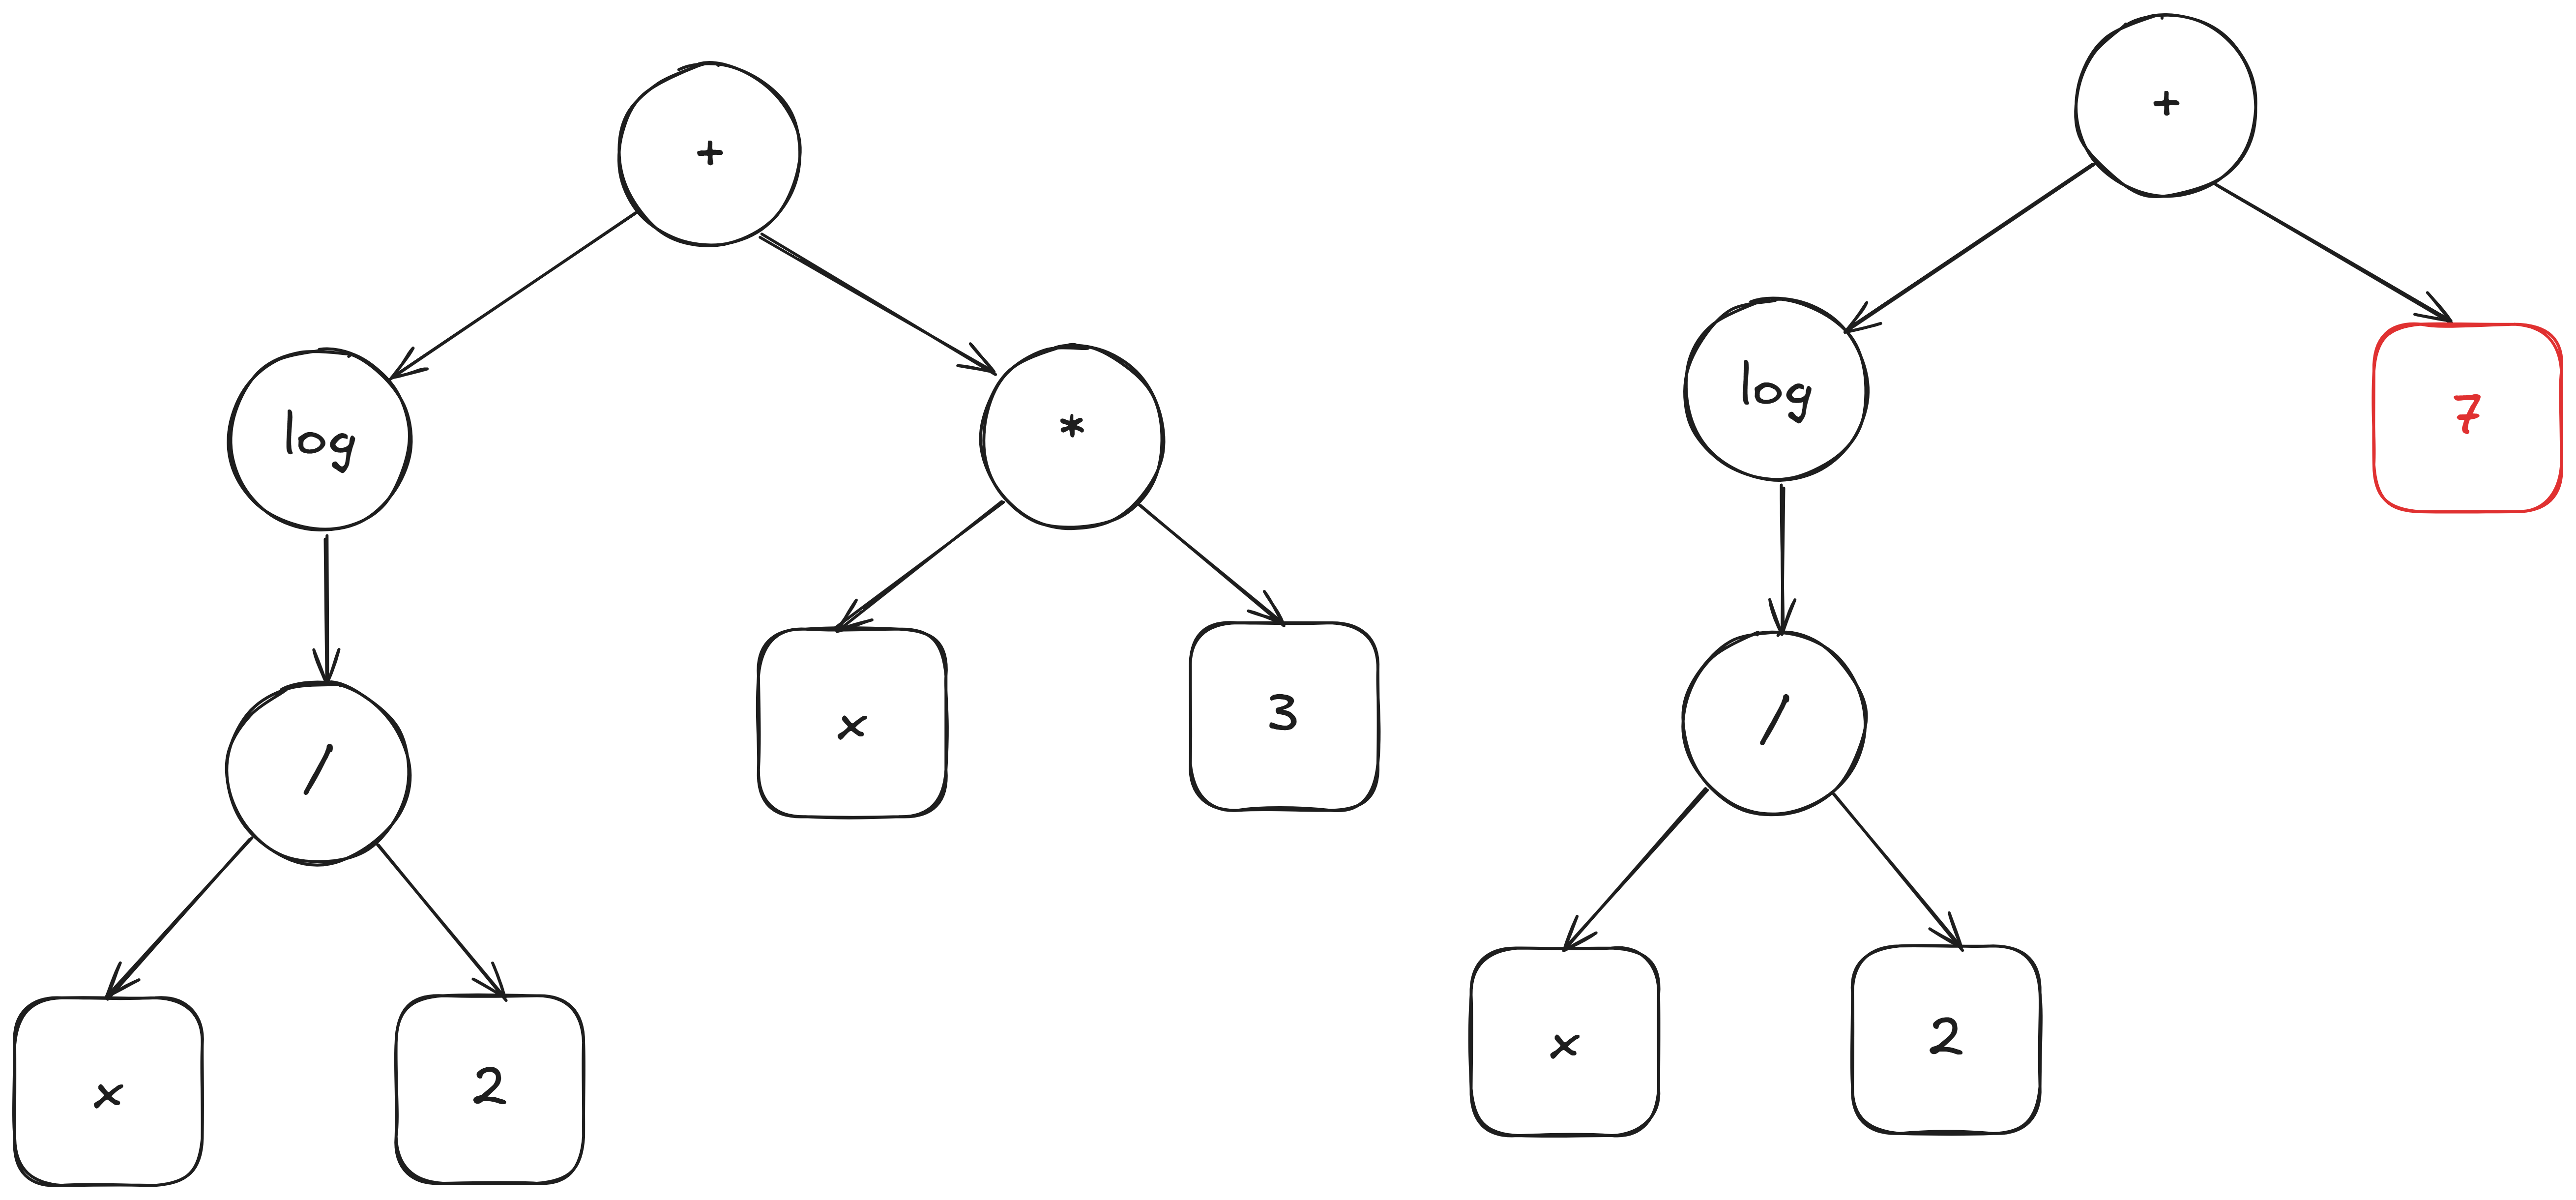
\includegraphics[width=0.5\textwidth]{images/ast_3_mutation.png}
  \label{fig:ast_mutation}
\end{figure}

É importante destacar que esse algoritmo não precisa necessariamente retornar uma única expressão. Um conjunto de expressões pode ser retornado, permitindo ao usuário escolher a que melhor se adequa às suas necessidades~\cite{Angelis2023}.

Apesar dos avanços recentes, a regressão simbólica ainda enfrenta vários desafios. A complexidade computacional decorrente do grande espaço de busca de expressões possíveis pode tornar o processo de evolução lento e ineficiente. Além disso, a interpretabilidade das expressões geradas pode ser comprometida quando elas se tornam excessivamente complexas, dificultando a compreensão por parte dos usuários finais~\cite{Angelis2023,sr_book}.

Além disso, a codificação de expressões como árvores pode levar o algoritmo de regressão a visitar expressões logicamente equivalentes várias vezes~\cite{eggp}. Por exemplo, as expressões $x + y$ e $y + x$ são logicamente iguais, mas seriam representadas por árvores diferentes. Testes empíricos indicam que apenas 40\% das expressões geradas por algoritmos genéticos para regressão simbólica são únicas~\cite{inefficiency_gp}.

\subsection{Saturação de igualdade para Regressão Simbólica}

Diante dos desafios enfrentados pela regressão simbólica tradicional, uma abordagem alternativa que tem ganhado destaque é o uso de grafos de igualdade (Equality Graphs - e-graphs) para representar e manipular expressões matemáticas~\cite{eggp,rEGGression}. E-graphs são estruturas de dados que armazenam múltiplas expressões equivalentes de forma compacta, permitindo a aplicação eficiente de transformações algébricas e simplificações nos indivíduos presentes no espaço de busca. Utilizando essa estrutura de dados, é possível realizar uma operação chamada de saturação de igualdade, que consiste em aplicar regras de reescrita para gerar todas as expressões logicamente equivalentes a uma dada expressão inicial.

\subsubsection{Grafos de Igualdade}

Grafos de igualdade são estruturas de dados que representam expressões matemáticas e suas equivalências de maneira eficiente~\cite{eggp,rEGGression}. Elementos matemáticos (operadores, variáveis e constantes) são representadas por e-nodes, enquanto classes de expressões equivalentes, ou seja, conjuntos de e-nodes equivalentes, são representadas por e-classes. Cada e-class contém um conjunto de e-nodes que representam diferentes formas de expressar a mesma expressão matemática. Cada e-node aponta para e-classes filhas, que representam os operandos da operação matemática representada pelo e-node, permitindo que variações de uma mesma expressão compartilhem subárvores e sejam representadas sem consumo elevado de memória.

A Figura \ref{fig:egraph_example} ilustra um grafo de igualdade. Note que as expressões $2x$ e $x + x$ pertencem à mesma e-class, uma vez que são logicamente equivalentes. A implementação de e-graphs utiliza uma estrutura union-find para gerenciar a união de e-classes quando novas equivalências são descobertas durante o processo de saturação~\cite{eggp}. Uma e-class armazena uma lista de e-nodes que pertencem a ela, uma lista de e-nodes pais (e-nodes que possuem essa e-class como filha) e demais informações auxiliares para otimizar operações de busca e união.

\begin{figure}
  \centering
  \caption{Exemplo de um grafo de igualdade, adaptado de~\cite{eggp}.}
  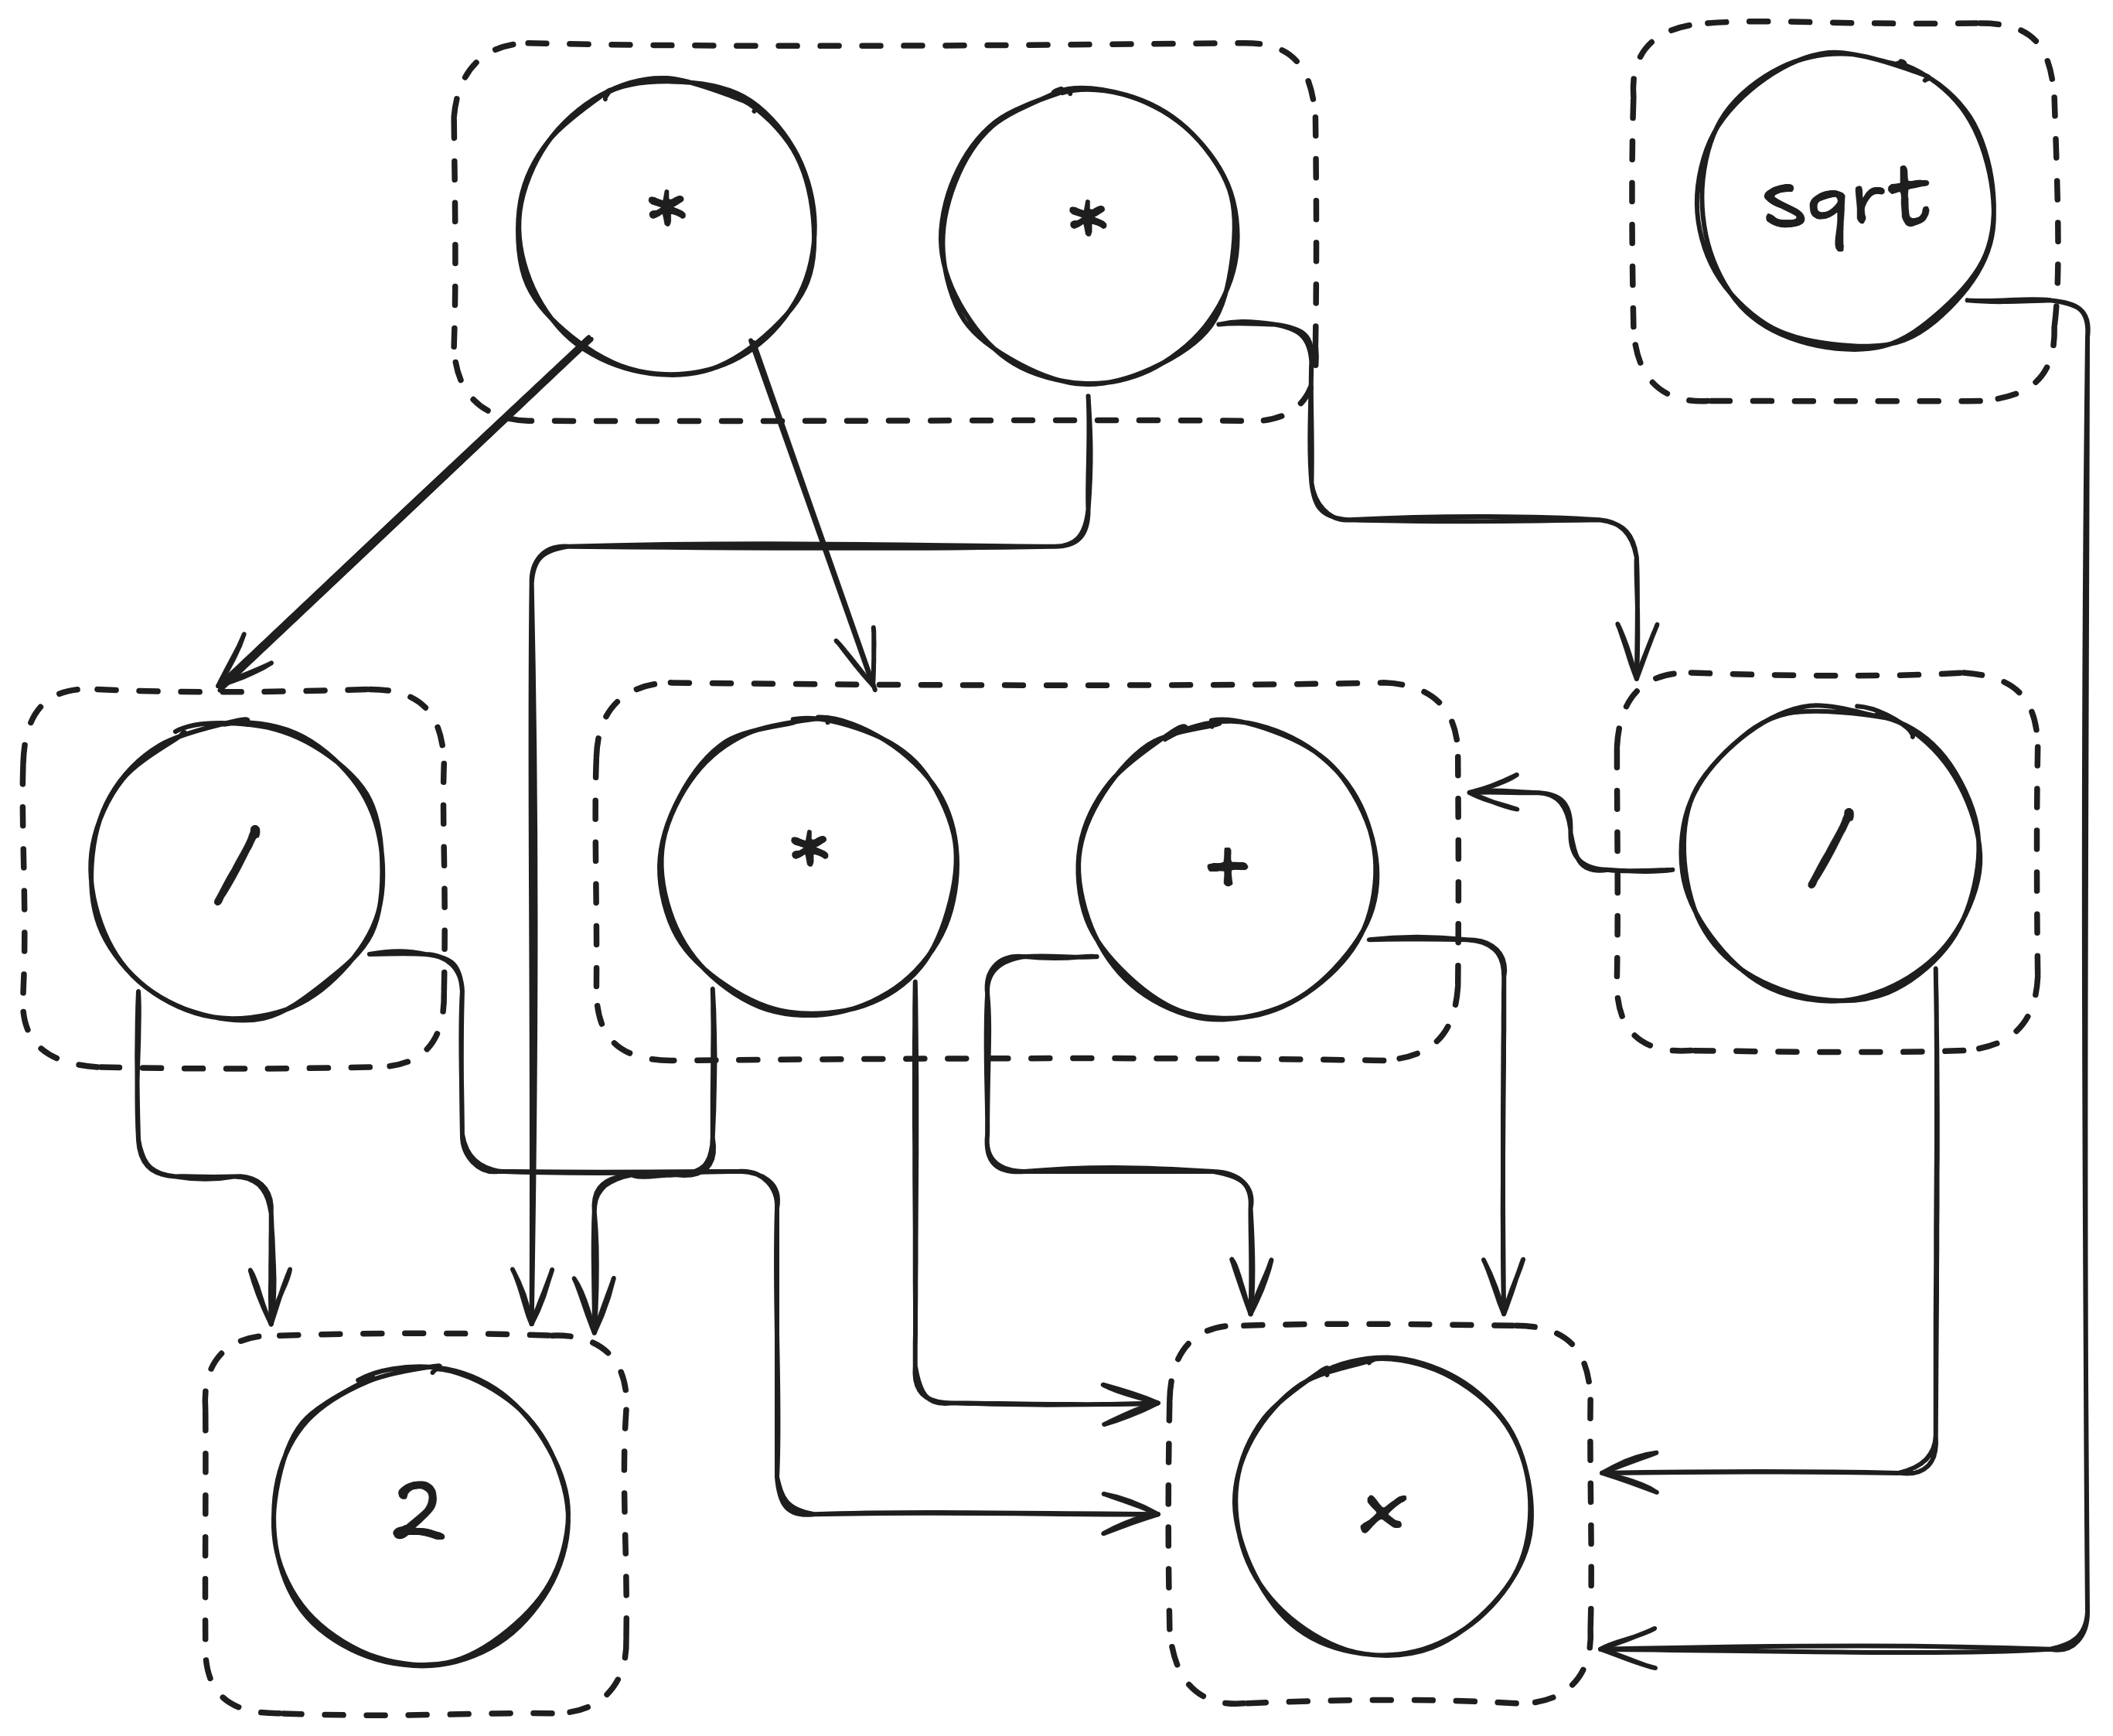
\includegraphics[width=0.7\textwidth]{images/egraph.png}
  \label{fig:egraph_example}
\end{figure}

\subsubsection{Saturação de igualdade}

Saturação de igualdade é o processo de aplicar regras de reescrita a uma árvore para gerar expressões logicamente equivalentes. Quando uma equivalência entre expressões é encontrada, as e-classes correspondentes são fundidas, sinalizando que diferentes caminhos estruturais possuem mesmo significado semântico. O processo é eficiente porque todas as regras de reescrita são aplicadas paralelamente~\cite{eggp}, utilizando a estrutura de e-graphs para evitar a duplicação de expressões. O processo se saturação acontece em quatro etapas:
\begin{enumerate}
  \item Elenque todas as regras de equivalência para o estado atual do e-graph;
  \item Aplique todas as regras;
  \item Junte e-classes equivalentes;
  \item Repita os passos anteriores até que nenhuma nova equivalência seja encontrada.
\end{enumerate}

Após a aplicação repetida de todas as regras, o e-graph é considerado saturado. Nesse estado, todas as expressões equivalentes possíveis foram geradas e armazenadas no e-graph.

\subsubsection{Algoritmo: eggp}

O algoritmo eggp (e-graph Genetic Programming) é uma implementação de um algoritmo genético para regressão simbólica que utiliza e-graphs e saturação de igualdade~\cite{eggp}. O algoritmo segue os passos tradicionais de um algoritmo genético, mas com algumas diferenças importantes:
\begin{enumerate}
  \item A cada nova expressão inserida no e-graph, é executada uma etapa de saturação, agrupando todas as expressões logicamente equivalentes;
  \item Os operadores de mutação e cruzamento são adaptados para geração de expressões não visitadas;
\end{enumerate}

Os operadores de mutação e cruzamento utilizam das informações do e-graph para gerar expressões ainda não visitadas. No cruzamento, uma subárvore aleatória de um dos pais é substituída por uma subárvore aleatória escolhida de um conjunto de todas as possíveis subárvores do outro pai. O conjunto é construído de tal forma que todos seus elementos, ao substituírem a subárvore original, geram expressões novas.

Na mutação, o processo tradicional é seguido, substituindo-se uma subárvore aleatória por uma nova subárvore gerada aleatoriamente. No entanto, caso a nova expressão já exista no e-graph, a subárvore é substituída por outra aleatória que faça parte do conjunto de símbolos de mesma aridade da subárvore original. Da mesma forma que no cruzamento, esse conjunto é formado de tal maneira que todas as substituições geram expressões novas.

Dessa forma, a utilização de grafos de igualdade reduz drasticamente o espaço de busca da regressão simbólica, permitindo maior eficiência do algoritmo sem aumento significativo no custo computacional. Durante o processo de evolução, é comum que expressões semanticamente equivalentes sejam geradas e exploradas~\cite{eggp,inefficiency_gp}. A utilização de e-graphs permite que esses caminhos repetidos dentro do espaço de soluções sejam podados do processo de busca, otimizando o algoritmo.

\subsection{Outros métodos para Regressão Simbólica}

Apesar de algoritmos genéticos serem os mais comuns para implementação de regressão simbólica, outros métodos podem ser utilizados~\cite{Bartlett_2024, Makke2024}:
\begin{enumerate}
    \item Aprendizado por reforço;
    \item Redes neurais;
    \item Transformadores.
\end{enumerate}

Para fins de comparação, esse trabalho também aborda uma implementação de regressão simbólica conhecida como Interação-Transformação~\cite{lsritr}, que utiliza uma abordagem diferente para geração de expressões matemáticas. Além disso, também será abordada uma técnica conhecida como Regressão Simbólica Exaustiva~\cite{Bartlett_2024}, que utiliza uma técnica similar à Interação-Transformação, mas que visa explorar todo o espaço de expressões possíveis dentro de um recorte delimitado, garantindo que a solução ótima seja encontrada.

\subsubsection{Interação-Transformação}

A regressão simbólica utilizando da estrutura de Interação-Transformação (IT) é uma abordagem que restringe o espaço de busca de expressões matemáticas para aquelas que podem ser representadas como uma combinação polinomial das variáveis seguidas por uma transformação não-linear~\cite{lsritr}. Diferentemente dos algoritmos genéticos, nessa implementação, algumas relações não podem ser representadas.

Nessa representação, os termos são representados por uma tupla $(\mathbf{P}, \mathbf{t})$, onde $\mathbf{P}$ é um vetor de expoentes e $\mathbf{t}$ é uma função de transformação sendo aplicada sobre os termos do polinômio~\cite{lsritr}. Como um exemplo dessa representação, considere uma regressão de quatro variáveis de entrada, $x_1$, $x_2$, $x_3$ e $x_4$. Considere que a função de transformação seja $t(x) = log(x)$. Então, teríamos a seguinte representação:

\begin{equation}
  \begin{aligned}
    \mathbf{T} &= (x_1, x_2, x_3, x_4) \\
    \mathbf{t_1} &= ([1, 0, 0, 0], log) \\
    \mathbf{t_2} &= ([0, 1, 0, 0], log) \\
    \mathbf{t_3} &= ([0, 0, 1, 0], log) \\
    \mathbf{t_4} &= ([0, 0, 0, 1], log)
  \end{aligned}
\end{equation}

Para gerar novas expressões, o algoritmo utiliza uma abordagem de busca em largura. A cada iteração, o algoritmo gera todos os termos possíveis decorrentes da combinação dos termos já existentes de forma que $t_k = (P_i + P_j, id)$ e $t_l = (P_i - P_j, id)$. No exemplo anterior, teríamos para a combinação de $t_1$ e $t_2$ os seguintes termos:

\begin{equation}
  \begin{aligned}
    \mathbf{t_5} &= ([1, 1, 0, 0], log) \\
    \mathbf{t_6} &= ([1, -1, 0, 0], log)
  \end{aligned}
\end{equation}

Para etapa de transformação, para cada termo $(\mathbf{P}, t)$, o algoritmo gera um novo termo $(\mathbf{P}, t')$ para cada função de transformação $t' != t$ disponível. No exemplo anterior, considerando que as funções de transformação disponíveis sejam $log$,  $sqrt$ e $e^x$, teríamos os seguintes termos:

\begin{equation}
  \begin{aligned}
    \mathbf{t_7} &= ([1, 0, 0, 0], sqrt) \\
    \mathbf{t_8} &= ([1, 0, 0, 0], e^x) \\
    \mathbf{t_9} &= ([0, 1, 0, 0], sqrt) \\
    \mathbf{t_{10}} &= ([0, 1, 0, 0], e^x) \\
    \mathbf{t_{11}} &= ([0, 0, 1, 0], sqrt) \\
    \mathbf{t_{12}} &= ([0, 0, 1, 0], e^x) \\
    \mathbf{t_{13}} &= ([0, 0, 0, 1], sqrt) \\
    \mathbf{t_{14}} &= ([0, 0, 0, 1], e^x) \\
    \mathbf{t_{15}} &= ([1, 1, 0, 0], sqrt) \\
    \mathbf{t_{16}} &= ([1, 1, 0, 0], e^x) \\
    \mathbf{t_{17}} &= ([1, -1, 0, 0], sqrt) \\
    \mathbf{t_{18}} &= ([1, -1, 0, 0], e^x)
  \end{aligned}
\end{equation}

Para cada expressão gerada, o algoritmo avalia a aptidão da expressão. Todas as expressões que não atingirem um valor mínimo de aptidão são descartadas~\cite{lsritr}.

\subsubsection{Regressão Simbólica Exaustiva}

Semelhantemente a regressão simbólica utilizando Interação-Transformação, a regressão simbólica exaustiva busca limitar o espaço de busca, mas com o objetivo de explorar todo o espaço, garantindo que a solução ótima seja encontrada~\cite{Bartlett_2024}.

Nessa abordagem, a geração de expressões é feita por meio da geração de todas as combinações possíveis entre operadores de aridade zero, um e dois. A aridade zero é representada por constantes, a aridade um por funções unárias (como $log$ e $sqrt$) e a aridade dois por funções binárias (como $+$, $-$, $*$ e $/$)~\cite{Bartlett_2024}. Considere uma árvore de profundidade máxima $d = 4$ e um conjunto de operadores de aridade zero ($x$), um ($f(x)$) e dois ($f(x_1, x_2)$). Nesse caso, temos apenas quatro árvores válidas, conforme ilustrado na Figura \ref{fig:exhaustive_example}.

\begin{figure}
  \centering
  \caption{Exemplo de árvores geradas por regressão simbólica exaustiva.}
  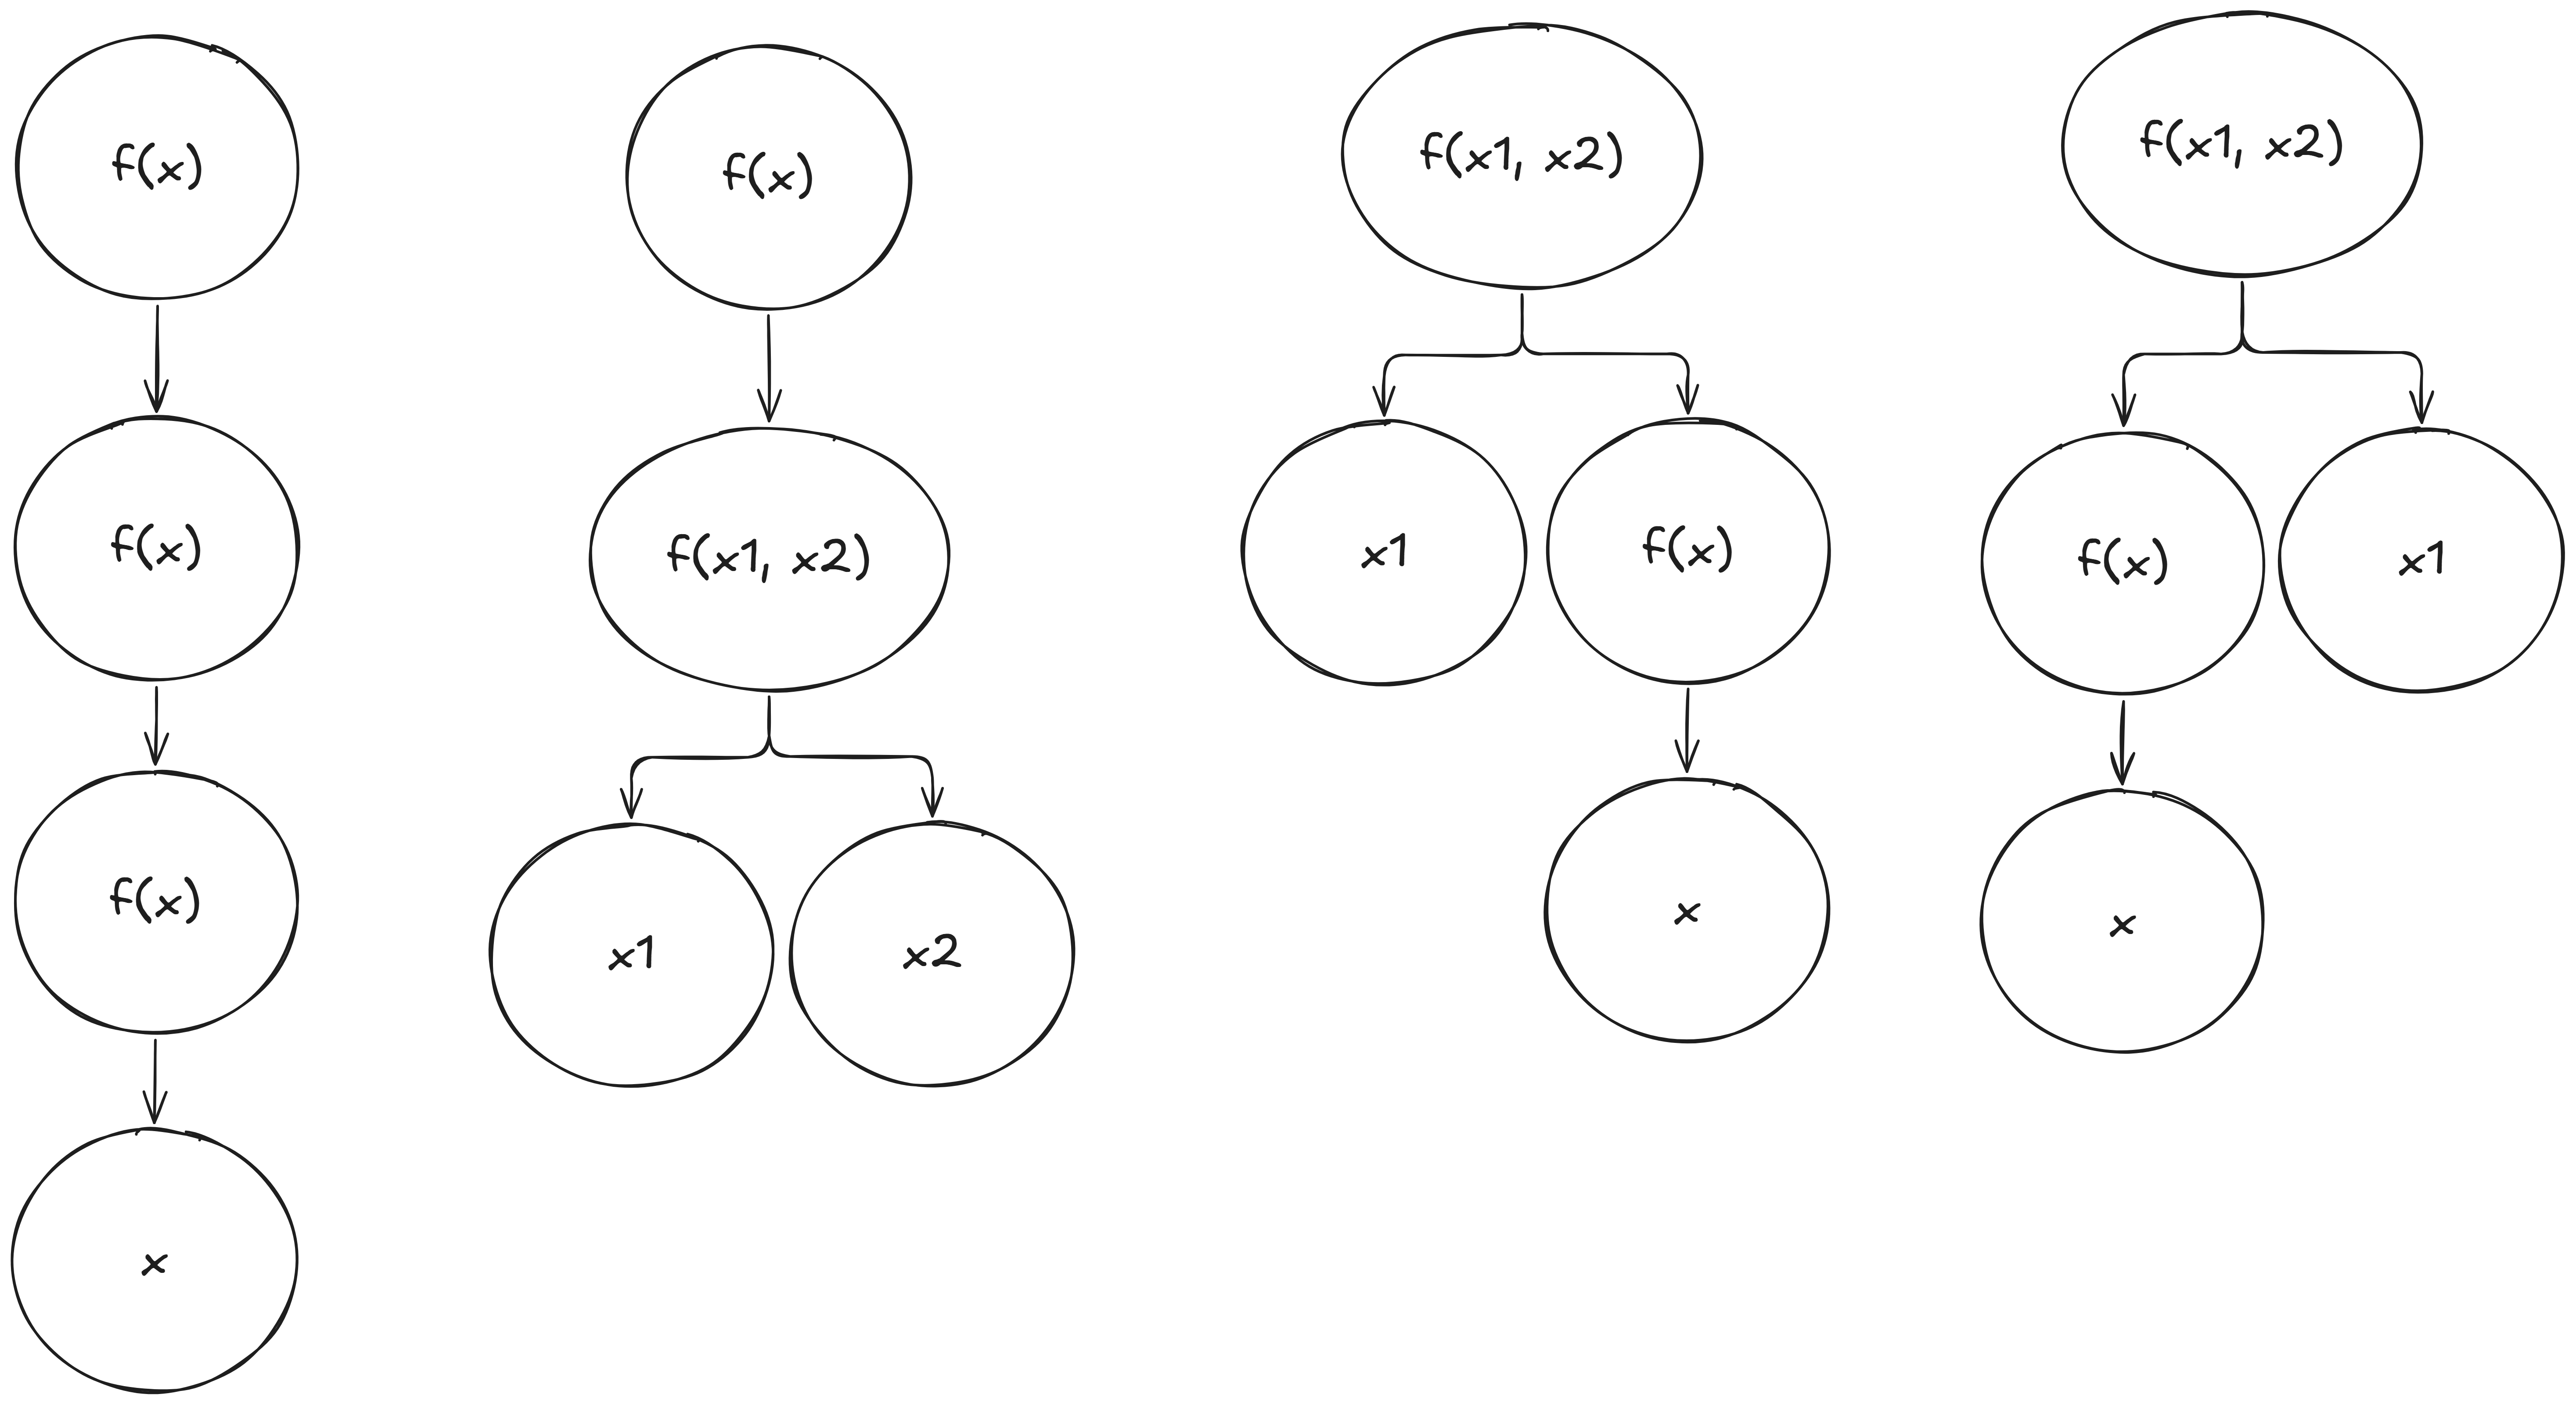
\includegraphics[width=0.8\textwidth]{images/exhaustive_example.png}
  \label{fig:exhaustive_example}
\end{figure}

Após a geração de todas as expressões, o algoritmo checa por expressões logicamente equivalentes, removendo-as do conjunto de expressões~\cite{Bartlett_2024}.

\section{Ferramentas para Regressão Simbólica}

Existem diversas ferramentas disponíveis para exploração de algoritmos de regressão simbólica. Essas ferramentas variam desde implementações comerciais até bibliotecas de código aberto, cada uma com suas próprias características e funcionalidades.

HeuristicLab é uma ferramenta gráfica que, dentre outros algoritmos, suporta a exploração de algoritmos de regressão simbólica. Ele permite a criação de algoritmos personalizados e a visualização dos resultados de forma interativa. A ferramenta é extensível e pode ser adaptada para diferentes necessidades de pesquisa~\cite{wagner2014architecture}. A ferramenta exibe a fronteira de Pareto final, detalhes estatísticos do modelo gerado, gráficos de desempenho e a representação final da árvore de busca.

Assim como a ferramenta anterior, TuringBot é uma interface gráfica para exploração de algoritmos de regressão simbólica. Ele mostra ao usuário as melhores expressões encontradas (fronteira de Pareto) para o conjunto de dados fornecido com algumas métricas simples do modelo criado~\cite{turingbot2020}.

Para além de ferramentas comerciais, existem diversas bibliotecas que permitem a exploração de algoritmos de regressão simbólica. No caso do algoritmo eggp, apresentado anteriormente, é possível utilizar a ferramenta \textit{rEGGression}~\cite{rEGGression} para explorar os modelos gerados por esse algoritmo. Essa ferramenta permite que as expressões encontradas pelo modelo sejam consultadas por tamanho, complexidade e número de parâmetros numéricos; permite a inserção de novas expressões; permite a listagem de sub-expressões; e permite o uso de padrões para busca de expressões~\cite{rEGGression}.

Apesar da existência de ferramentas que permitem exploração de modelos de regressão simbólica, poucas ferramentas permitem a criação de \textit{pipelines} de dados para criação de modelos preditivos. As ferramentas disponíveis também não permitem a exploração de padrões dentro das expressões geradas.

\section{Conclusão}

A revisão de literatura apresentada neste capítulo retoma os principais conceitos e técnicas relacionados à regressão simbólica, incluindo algoritmos genéticos, programação genética e o uso de grafos de igualdade, dentre outras técnicas. Além disso, foram apresentadas ferramentas e implementações que permitem a exploração desses conceitos na prática. Nos próximos capítulos, será apresentada uma proposta de ambiente de exploração de algoritmos de regressão simbólica, com foco na implementação do algoritmo eggp e na utilização de grafos de igualdade para otimização do processo de evolução de expressões matemáticas.
